\documentclass[11pt,a4paper,oneside]{article}
\usepackage[latin1]{inputenc}
\usepackage{amsmath}
\usepackage{amsfonts}
\usepackage{amssymb}
\usepackage{graphicx}
\usepackage{color}
\usepackage {tikz}
\usetikzlibrary {er}
\usepackage[left=2.00cm, right=2.00cm, top=1.00cm]{geometry}
\graphicspath{{./}}

\begin{document}
	\title{DS 221 - Introduction to Scalable Systems \\ Parallelization of KMeans Clustering using OpenMP}
	\author{Shriram R. \\ M Tech (CDS) \\ 06-02-01-10-51-18-1-15763}
	\maketitle
	
	\section{Introduction}
	KMeans Clustering algorithm has been parallelized using OpenMP and the speedup for different thread count and schedule configurations were observed through experiments. The following sections cover the methodology, experimental setup and results in detail.
	
	\section{Methodology}
	The algorithm runs for a fixed no. of iterations (currently 100) for convergence of centroids. The following steps are followed in each iteration,
	\begin{enumerate}
		\item A parallel region with given no. of threads is started with the points, centroid, label and temp array in shared mode. The temp array is used to store updated centroid info for each thread
		\begin{enumerate}
		\item The set of points is distributed among the threads using either static or dynamic chunks
		\item Each thread will assign its points to their respective nearest centroid by computing euclidean distance and update the corresponding entry in label array
		\item The threads also update the temp array with its local cluster size and centroid value
	    \end{enumerate}
		\item Global centroid information is updated by aggregating the thread level centroids computed in the previous step and is used for the next iteration
	\end{enumerate}
    The above methodology is illustrated in the code snippet in appendix A.
	
	
	\section{Experimental Setup}
	The Turing compute cluster having 24 nodes with 8 cores each was used to run the experiments. Batch job was created and executed using PBS. For each thread count, two experiments (i.e) one with static and dynamic chunk sizes were performed. \\
	\newline
	The time taken to run the KMeans clustering was measured using C library function and was printed to stdout. Each experiment was repeated 20 times and then the average was computed for the plots and analysis. \\
	\newline
	\begin{verbatim}
	
	
			
				
	
	\end{verbatim}
	
	\section{Results}
	
	  \begin{center}
		\begin{tabular}{|l|c|c|c|c|}
			\hline 
			\textbf{Schedule} & \textbf{Threads}  & \textbf{Sequential (Avg.) (s)} & \textbf{Parallel (Avg.) (s)} & \textbf{Speedup} \\
			\hline
		    Static & 4 &  0.36895 & 0.20875 & 1.77\\ 
			\hline 
		     Static & 8 &  0.3715 & 0.15455 & 2.40\\
			\hline 
			 Static & 16 &  0.38465 & 0.10405 & 3.70\\
			\hline 
			 Dynamic & 4 &  0.37980 & 0.10150 & 2.10\\ 
			\hline 
			Dynamic & 8 &  0.36990 & 0.10600 & 3.49 \\
			\hline 
			Dynamic & 16 &  0.37090 & 0.06345 & 5.85\\
			\hline 
		\end{tabular}
	\end{center}
	
	\begin{center}
		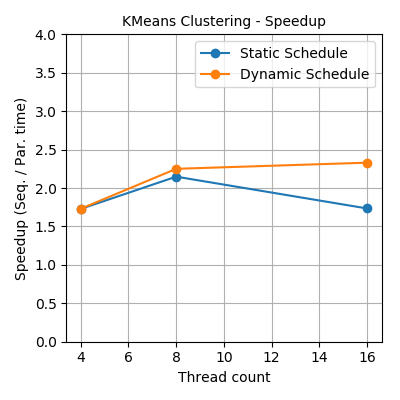
\includegraphics[scale=0.7]{1.png}		
	\end{center}

    \begin{center}
    	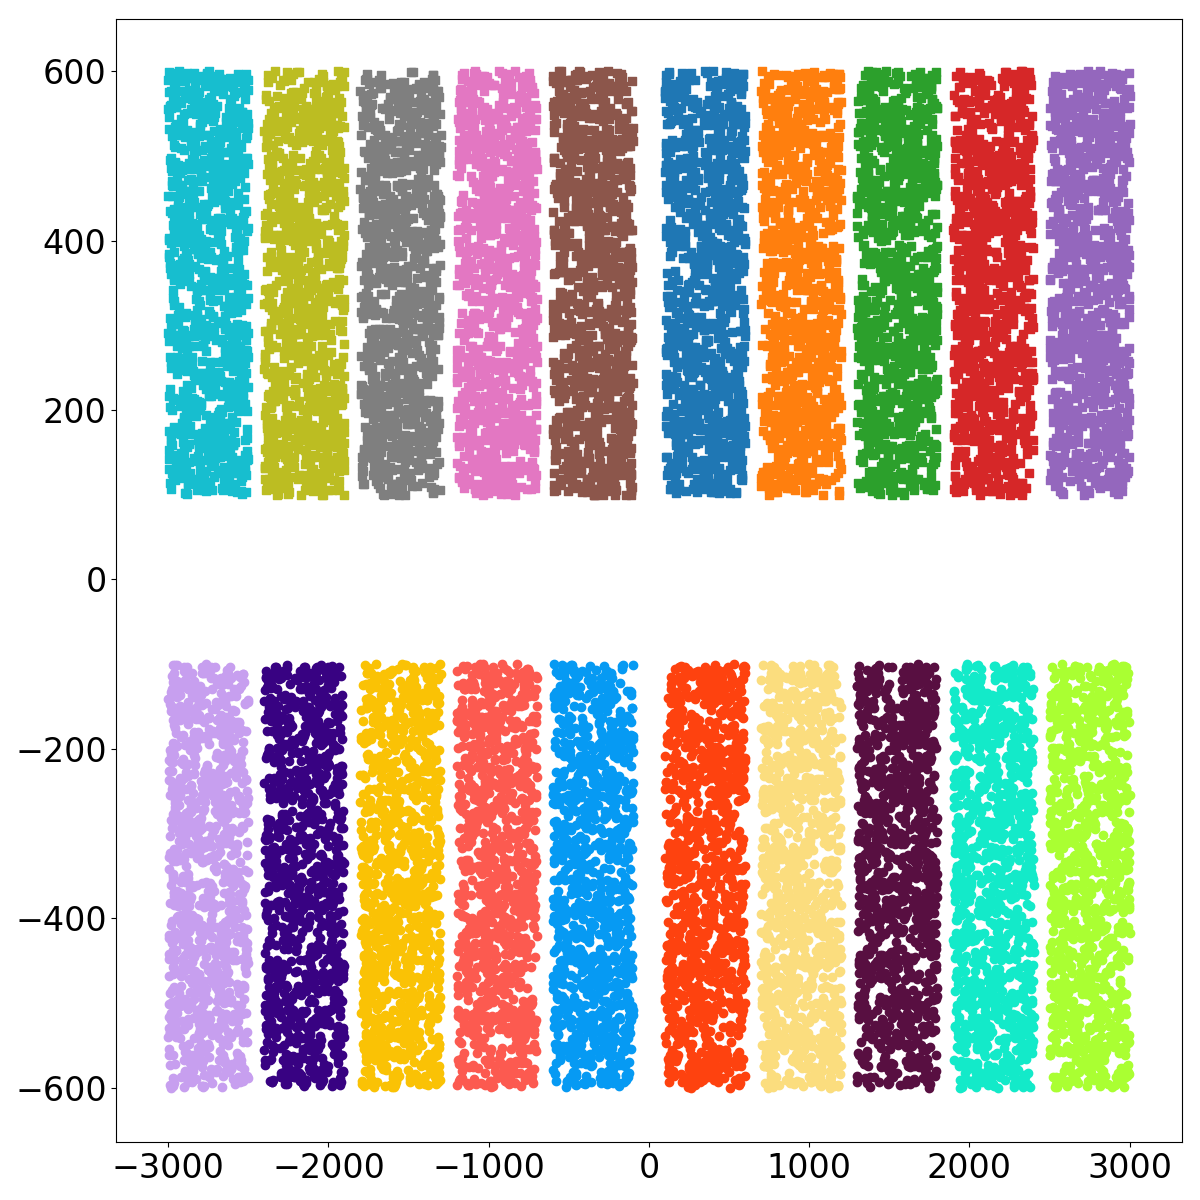
\includegraphics[scale=0.2]{2.png}	\\
    	20 Clusters	
    \end{center}
	 
     
    \section{Observations}
    It can be observed that the speedup increases with no. of threads. Also, the increase is not strictly linear as seen in the plot. Dynamic scheduling was more efficient than static due to its excellent cache and balance properties. There is a considerable amount of overhead in creating the threads for each iteration and so the speedup for P threads is quites less than P.
     
    
    \section{References}
    \begin{list}{}{}
    	\item 1. https://en.cppreference.com/w/c
    	\item 2. DS 221 Course lecture notes
    	\item 3. https://computing.llnl.gov/tutorials/openMP/
    	\item 4. http://www.arc.ox.ac.uk/content/pbs-job-scheduler
    	\item 5. https://www.dartmouth.edu/~rc/classes/intro\_openmp/print\_pages.shtml
    \end{list}

    \section{Appendix A} 
    
    \begin{verbatim}
    for (int i = 0; i < ITER; i++)
    {	
    // Parallel region
    #pragma omp parallel num_threads(THREADS) shared(pts, label, centroid, temp)
    {	
    float min_dist, dist;
    int tid, min_label;
    tid = omp_get_thread_num();
    
    // Reset temp
    for (int k = 0; k < CLUSTERS; k++)
    {
    temp[tid][k][0] = 0;
    temp[tid][k][1] = 0;
    temp[tid][k][2] = 0;
    }
    
    // Assign Labels for all points
    #pragma omp for schedule(static, chunk)
    for (int j = 0; j < SIZE; j++)
    {
    min_dist = FLT_MAX;                
    for (int k = 0; k < CLUSTERS; k++)
    {
    dist = (pts[j][0] - centroid[k][0]) * (pts[j][0] - centroid[k][0]) +
    (pts[j][1] - centroid[k][1]) * (pts[j][1] - centroid[k][1]);
    if (dist < min_dist)
    {
    min_dist = dist;
    min_label = k;
    }
    }
    label[j] = min_label;
    temp[tid][min_label][0] += pts[j][0];
    temp[tid][min_label][1] += pts[j][1];
    temp[tid][min_label][2] += 1; 
    }
    }
    // End of parallel region
    
    // Collect temp
    for (int j = 1; j < THREADS; j++)
    {
    for (int k = 0; k < CLUSTERS; k++)
    {
    temp[0][k][0] += temp[j][k][0];
    temp[0][k][1] += temp[j][k][1];
    temp[0][k][2] += temp[j][k][2];
    }
    }
    
    // Compute and update centroid
    for (int k = 0; k < CLUSTERS; k++)
    {
    if (temp[0][k][2] == 0)
    continue;
    centroid[k][0] = temp[0][k][0] / temp[0][k][2];
    centroid[k][1] = temp[0][k][1] / temp[0][k][2];
    }
    }
    \end{verbatim}
    
\end{document}